\section{Extended Proxy CAM} \label{sec:iproxy_cam}

To solve the problem described in Section~\ref{sec:problem},
we extended our previous work.
The new design is called Extended Proxy CAM.
We want to make the system compatible with original CA service,
but due to some security reason, the compatibility is still under pursuit.
The new WIP design is based on the ETSI standard ITS,
it should be easy to apply this design to other ITS standards.
The current preliminary design is described in this section.

\subsection{System design}

\begin{figure}[htbp]
    \begin{center}
        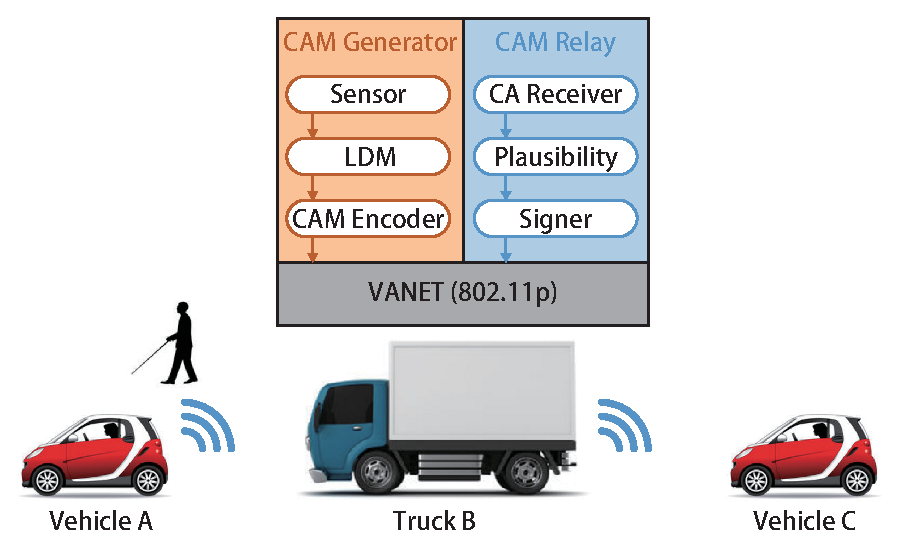
\includegraphics[width=0.85\linewidth]{figures/exProxyCAM.eps}
        \caption{System design}
        \label{fig:system_design}
    \end{center}
\end{figure}

Figure~\ref{fig:system_design} shows the overview of the system design.
Our previous work is limited to RSU, but the new design should also be applicable to moving vehicles, such as large trucks.

ITS enabled vehicles are usually equipped with sensors to detect the pedestrian
and other vehicles or objects in its surrounding within the visual field.
Then record the data in LDM.
When the system is deployed on vehicles, we can utilize the LDM instead of harvesting data directly from sensors.

For those non-ITS enabled road users,
we can directly use the information from LDM to generate CAMs for them.
Then the system broadcasts the generated CAMs to its surrounding ITS-Ss.
Upon receiving the CAMs, we can process the message just like normal CAMs,
storing the information into their own LDMs.

For those ITS enabled road users,
when the CAMs could suffer serious loss due to the large vehicle or other kinds of obstacles with this system deployed,
the system should relay the CAMs in a manner described as follows.
First, upon the obstacles receiving the CAM, we need to check the plausibility of it,
using similar techniques described in Section~\ref{sec:related_works}, to ensure the sender is not a malicious one.
Only if it passed the plausibility check, the intermediate vehicle, as shown in Figure~\ref{fig:system_design},
should append its signature and public key to the CAM, then relay the CAM to its surrounding vehicles.

In the following sections, we describe the system in detail.
The whole system can be split into two part, CAM generator, and CA relay.

\subsubsection{CAM generator}

The CAM generator generates the necessary CAMs for those non-ITS enabled road users.
It is based on our previous work. Because our new design could be deployed to vehicles,
we could save sensors if the system is installed on a vehicle.
The system could use the data in LDM on the vehicle to provide more detailed information (lane position, car type, etc.).
It's easy to distinguish those non-ITS enabled vehicles in LDM.
Additionally, we can generate CAMs for other on road objects which could endanger the road traffic.
If we could identify the vehicle's ID from sensors,
we should assign an ID connected with it to the corresponding object in LDM.
Otherwise, a random ID is assigned.
Object tracking techniques should be used to ensure that we assign the same object with the same ID.

As shown in Figure~\ref{fig:system_design}, when the truck B recognize a walking man with its sensors,
which is apparently a non-ITS enabled road user,
it firstly records the data into its LDM and assigned a random ID to it.
Vehicle C cannot perceive the existence of this walking man because truck B blocks the view of its sensors.
Then the CAM encoder on truck B collect the information from its LDM to generate CAM for this walking man,
then broadcast the CAM to its surrounding vehicles.
Therefore, vehicle C knows there is a collision risk with the walking man if it overtakes truck B.
At the same time, with object tracking techniques,
truck B constantly tracks the walking man, and update the information in its LDM. 

\subsubsection{CA relay}

We use CA relay to overcome the issue described in Section~\ref{sec:problem},
large vehicles could interfere the V2V wireless communications, resulting in CAMs losses.
CA relay is used to relay the CAMs from surrounding vehicles to surrounding vehicles.
As shown in Figure~\ref{fig:system_design},
the V2V communication between vehicle A and vehicle C could suffer serious loss due to the truck B blocking the signal.
Under such scenario, it could be dangerous if vehicle C decide to overtake truck B from behind.
We use the truck B as an intermediate station to relay the CAMs from vehicle A.
Upon truck B receiving CAM from vehicle A, it firstly conducts a plausibility check,
to ensure the CAM is not from a malicious sender.
If passed the check,
it should sign-off the CAM using its own private key and append its public key to the CAM then broadcast the signed CAM.

Upon receiving a relayed CAM, the receiver should firstly check the signature of the message,
then it should conduct a plausibility check if the intermediate node is a vehicle.
Only if the CAM passed all checks, we can consider the CAM is a valid one.

\begin{figure}[htbp]
    \begin{center}
        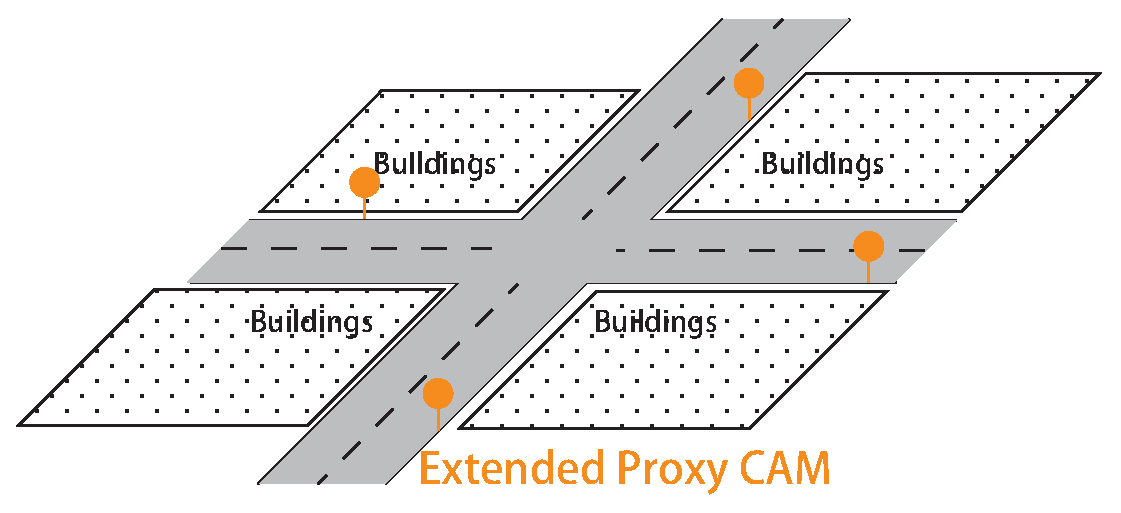
\includegraphics[width=0.85\linewidth]{figures/crossroad.eps}
        \caption{Crossroad scenario}
        \label{fig:crossroad}
    \end{center}
\end{figure}

Such system should also be applicable to RSUs.
Figure~\ref{fig:crossroad} describes a scenario which is common in Japan~\cite{tsugawa2011current},
in where some streets are narrow, and the buildings block the view at crossroads.
Drivers always have to stop at each crossroad to ensure it is safe to pass.
Even with ITS, the V2V communication still could be blocked by the buildings.
If we place some RSUs with our system on each side of the crossroad and connect them to each other to generate and relay the CAM,
the vehicle could have a better perception of other vehicles.

\subsection{Considerations}

Currently, this design is still not completed yet.
To improve the security of this system,
when deployed on vehicles,
the system should only be deployed those which could endanger the road safety and also under serious supervision,
such as trucks, buses and etc.
Because there is a risk, that an attacker could manipulate the CAM to attack the network,
so it is not safe to deploy such system to normal vehicles.